\documentclass[border=8pt]{standalone}
\usepackage[T1]{fontenc}\usepackage{helvet}\renewcommand{\familydefault}{\sfdefault}
\usepackage{tikz}\usetikzlibrary{arrows.meta, positioning, calc, backgrounds}
\definecolor{ink}{HTML}{1a1916}
\definecolor{inktwo}{HTML}{3a3a35}
\definecolor{inkthree}{HTML}{6a6862}
\definecolor{rule}{HTML}{b8b09a}
\definecolor{amber}{HTML}{a8730a}
\definecolor{red}{HTML}{c8261a}
\definecolor{paper}{HTML}{f0eee5}
\definecolor{slab}{HTML}{d8d4c6}
\tikzset{
  >={Stealth[length=2.2mm]},
  wire/.style={line width=0.8pt, ink},
  modwire/.style={line width=0.6pt, dashed, ink},
  tastewire/.style={line width=0.6pt, dashed, amber},
  gatewire/.style={line width=0.6pt, dotted, ink},
  block/.style={rectangle, draw=ink, line width=0.9pt, fill=slab, minimum width=3.0cm, minimum height=1.9cm, inner sep=0pt},
  perf/.style={rectangle, draw=ink, line width=0.7pt, minimum width=3.0cm, minimum height=0.7cm, inner sep=2pt, font=\footnotesize, text=ink},
  title/.style={font=\scriptsize\bfseries, text=ink, anchor=north, inner sep=2pt},
  jack/.style={circle, draw=ink, fill=paper, line width=0.5pt, minimum size=3.2pt, inner sep=0pt},
  plabel/.style={font=\tiny, text=inktwo, anchor=west, inner sep=1pt},
  olabel/.style={font=\tiny, text=inktwo, anchor=east, inner sep=1pt},
  settings/.style={font=\scriptsize, text=ink, align=left, anchor=north west, inner sep=1pt, text width=2.9cm},
}
\begin{document}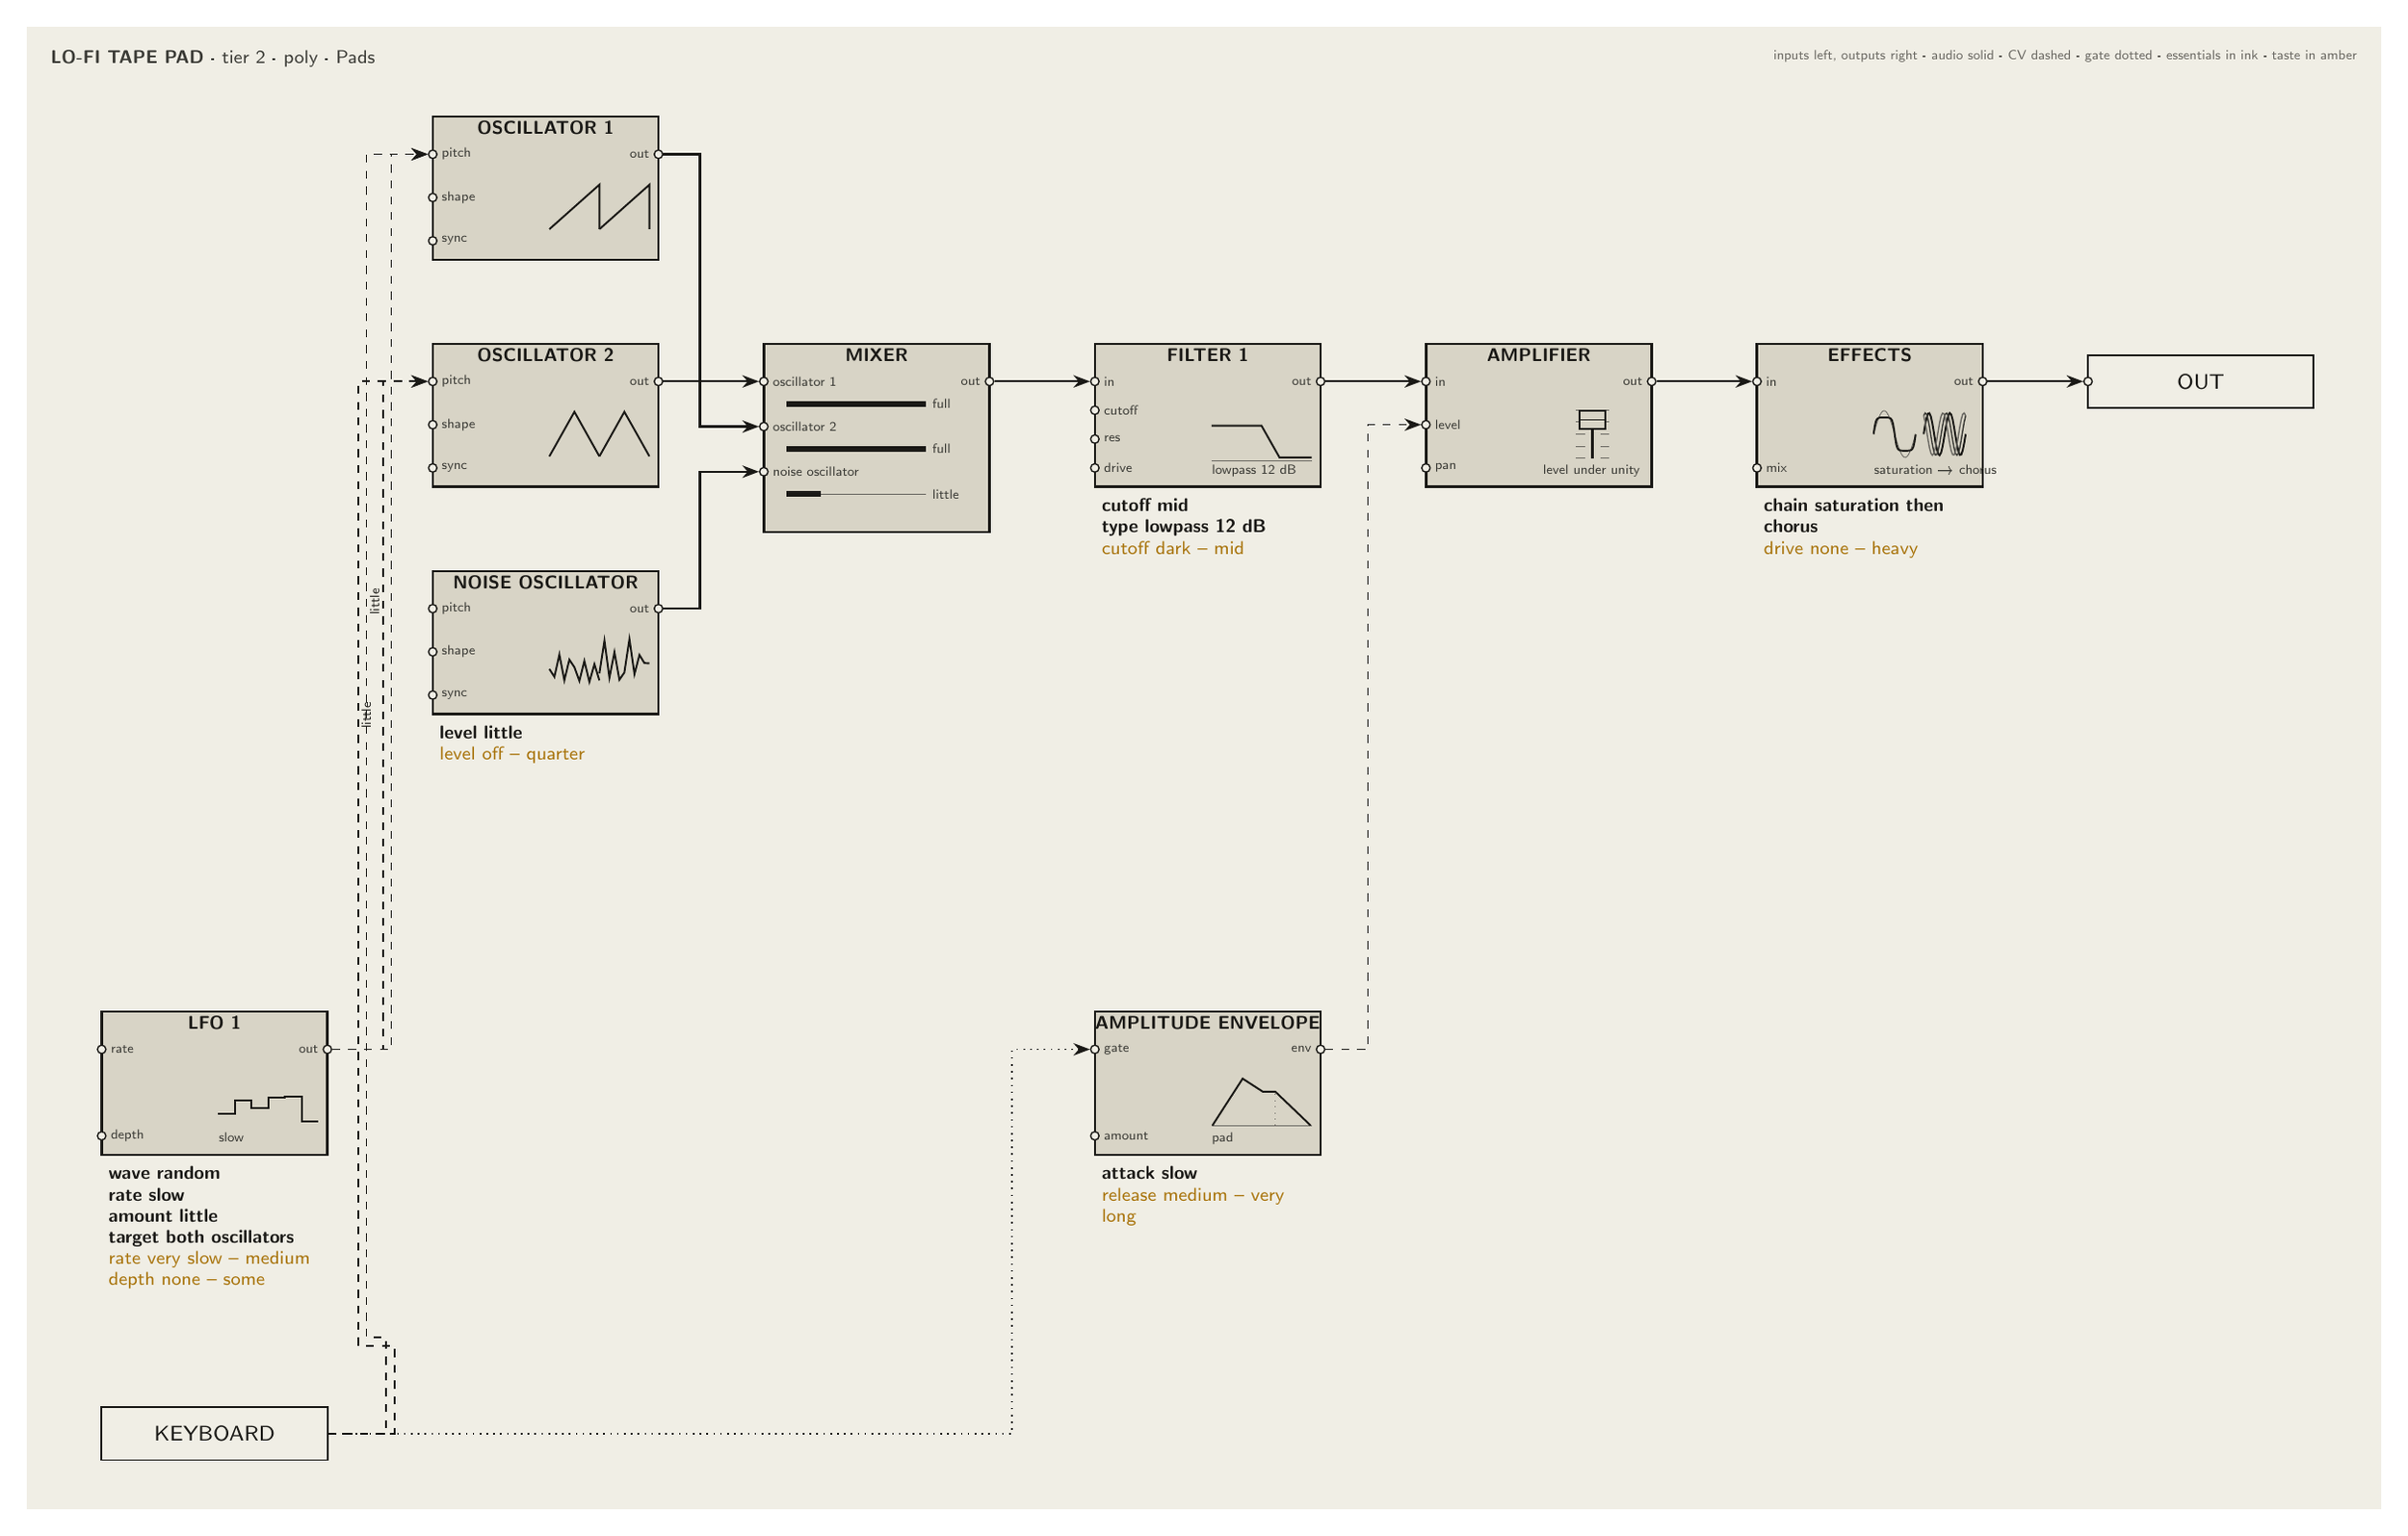
\begin{tikzpicture}
\begin{scope}[on background layer]\fill[paper] (-2.5,-14.539999999999997) rectangle (28.8,5.17);\end{scope}
\node[block, minimum height=1.9cm] (osc1) at (4.4,3.02) {};
\node[title] at (osc1.north) {OSCILLATOR 1};
\node[jack] (osc1-pitch) at (2.9000000000000004,3.4699999999999998) {};
\node[plabel] at (2.9800000000000004,3.4699999999999998) {pitch};
\node[jack] (osc1-shape) at (2.9000000000000004,2.8949999999999996) {};
\node[plabel] at (2.9800000000000004,2.8949999999999996) {shape};
\node[jack] (osc1-sync) at (2.9000000000000004,2.32) {};
\node[plabel] at (2.9800000000000004,2.32) {sync};
\node[jack] (osc1-out) at (5.9,3.4699999999999998) {};
\node[olabel] at (5.82,3.4699999999999998) {out};
\begin{scope}
\draw[ink, line width=0.7pt] (4.450,2.474) -- (5.115,3.066) -- (5.115,2.474);
\draw[ink, line width=0.7pt] (5.115,2.474) -- (5.780,3.066) -- (5.780,2.474);
\end{scope}
\node[block, minimum height=1.9cm] (osc2) at (4.4,0.0) {};
\node[title] at (osc2.north) {OSCILLATOR 2};
\node[jack] (osc2-pitch) at (2.9000000000000004,0.44999999999999996) {};
\node[plabel] at (2.9800000000000004,0.44999999999999996) {pitch};
\node[jack] (osc2-shape) at (2.9000000000000004,-0.125) {};
\node[plabel] at (2.9800000000000004,-0.125) {shape};
\node[jack] (osc2-sync) at (2.9000000000000004,-0.7) {};
\node[plabel] at (2.9800000000000004,-0.7) {sync};
\node[jack] (osc2-out) at (5.9,0.44999999999999996) {};
\node[olabel] at (5.82,0.44999999999999996) {out};
\begin{scope}
\draw[ink, line width=0.7pt] (4.450,-0.546) -- (4.783,0.046) -- (5.115,-0.546);
\draw[ink, line width=0.7pt] (5.115,-0.546) -- (5.447,0.046) -- (5.780,-0.546);
\end{scope}
\node[block, minimum height=1.9cm] (noise) at (4.4,-3.02) {};
\node[title] at (noise.north) {NOISE OSCILLATOR};
\node[jack] (noise-pitch) at (2.9000000000000004,-2.5700000000000003) {};
\node[plabel] at (2.9800000000000004,-2.5700000000000003) {pitch};
\node[jack] (noise-shape) at (2.9000000000000004,-3.1450000000000005) {};
\node[plabel] at (2.9800000000000004,-3.1450000000000005) {shape};
\node[jack] (noise-sync) at (2.9000000000000004,-3.72) {};
\node[plabel] at (2.9800000000000004,-3.72) {sync};
\node[jack] (noise-out) at (5.9,-2.5700000000000003) {};
\node[olabel] at (5.82,-2.5700000000000003) {out};
\begin{scope}
\draw[ink, line width=0.7pt] (4.450,-3.374) -- (4.517,-3.477) -- (4.583,-3.181) -- (4.649,-3.523) -- (4.716,-3.249) -- (4.783,-3.350) -- (4.849,-3.532) -- (4.915,-3.266) -- (4.982,-3.544) -- (5.049,-3.309) -- (5.115,-3.525);
\draw[ink, line width=0.7pt] (5.115,-3.432) -- (5.182,-2.996) -- (5.248,-3.491) -- (5.315,-3.149) -- (5.381,-3.516) -- (5.447,-3.420) -- (5.514,-2.975) -- (5.581,-3.442) -- (5.647,-3.186) -- (5.713,-3.294) -- (5.780,-3.298);
\end{scope}
\node[settings] at (2.95,-4.09) {\textbf{level little} \\ \textcolor{amber}{level off -- quarter}};
\node[block, minimum height=2.5cm] (mix) at (8.8,-0.30000000000000004) {};
\node[title] at (mix.north) {MIXER};
\node[jack] (mix-osc1) at (7.300000000000001,0.44999999999999996) {};
\node[plabel] at (7.380000000000001,0.44999999999999996) {oscillator 1};
\draw[inkthree, line width=0.3pt] (7.600,0.150) -- (9.450,0.150);
\draw[ink, line width=2.2pt] (7.600,0.150) -- (9.450,0.150);
\node[font=\tiny, text=inktwo, anchor=west, inner sep=1pt] at (9.500,0.150) {full};
\node[jack] (mix-osc2) at (7.300000000000001,-0.15000000000000002) {};
\node[plabel] at (7.380000000000001,-0.15000000000000002) {oscillator 2};
\draw[inkthree, line width=0.3pt] (7.600,-0.450) -- (9.450,-0.450);
\draw[ink, line width=2.2pt] (7.600,-0.450) -- (9.450,-0.450);
\node[font=\tiny, text=inktwo, anchor=west, inner sep=1pt] at (9.500,-0.450) {full};
\node[jack] (mix-noise) at (7.300000000000001,-0.75) {};
\node[plabel] at (7.380000000000001,-0.75) {noise oscillator};
\draw[inkthree, line width=0.3pt] (7.600,-1.050) -- (9.450,-1.050);
\draw[ink, line width=2.2pt] (7.600,-1.050) -- (8.062,-1.050);
\node[font=\tiny, text=inktwo, anchor=west, inner sep=1pt] at (9.500,-1.050) {little};
\node[jack] (mix-out) at (10.3,0.44999999999999996) {};
\node[olabel] at (10.22,0.44999999999999996) {out};
\node[block, minimum height=1.9cm] (filter1) at (13.200000000000001,0.0) {};
\node[title] at (filter1.north) {FILTER 1};
\node[jack] (filter1-in) at (11.700000000000001,0.44999999999999996) {};
\node[plabel] at (11.780000000000001,0.44999999999999996) {in};
\node[jack] (filter1-cutoff) at (11.700000000000001,0.06666666666666665) {};
\node[plabel] at (11.780000000000001,0.06666666666666665) {cutoff};
\node[jack] (filter1-res) at (11.700000000000001,-0.31666666666666665) {};
\node[plabel] at (11.780000000000001,-0.31666666666666665) {res};
\node[jack] (filter1-drive) at (11.700000000000001,-0.7) {};
\node[plabel] at (11.780000000000001,-0.7) {drive};
\node[jack] (filter1-out) at (14.700000000000001,0.44999999999999996) {};
\node[olabel] at (14.620000000000001,0.44999999999999996) {out};
\begin{scope}
\draw[inkthree, line width=0.3pt] (13.250,-0.605) -- (14.580,-0.605);
\draw[ink, line width=0.7pt] (13.250,-0.139) -- (13.915,-0.139) -- (14.154,-0.561) -- (14.580,-0.561);
\node[font=\tiny, text=inktwo, anchor=north west, inner sep=0pt] at (13.250,-0.650) {lowpass 12 dB};
\end{scope}
\node[settings] at (11.750000000000002,-1.0699999999999998) {\textbf{cutoff mid} \\ \textbf{type lowpass 12 dB} \\ \textcolor{amber}{cutoff dark -- mid}};
\node[block, minimum height=1.9cm] (amp) at (17.6,0.0) {};
\node[title] at (amp.north) {AMPLIFIER};
\node[jack] (amp-in) at (16.1,0.44999999999999996) {};
\node[plabel] at (16.18,0.44999999999999996) {in};
\node[jack] (amp-level) at (16.1,-0.125) {};
\node[plabel] at (16.18,-0.125) {level};
\node[jack] (amp-pan) at (16.1,-0.7) {};
\node[plabel] at (16.18,-0.7) {pan};
\node[jack] (amp-out) at (19.1,0.44999999999999996) {};
\node[olabel] at (19.020000000000003,0.44999999999999996) {out};
\begin{scope}
\draw[ink, line width=1.2pt] (18.315,-0.570) -- (18.315,0.070);
\draw[inkthree, line width=0.3pt] (18.095,-0.570) -- (18.215,-0.570) (18.415,-0.570) -- (18.535,-0.570);
\draw[inkthree, line width=0.3pt] (18.095,-0.410) -- (18.215,-0.410) (18.415,-0.410) -- (18.535,-0.410);
\draw[inkthree, line width=0.3pt] (18.095,-0.250) -- (18.215,-0.250) (18.415,-0.250) -- (18.535,-0.250);
\draw[inkthree, line width=0.3pt] (18.095,-0.090) -- (18.215,-0.090) (18.415,-0.090) -- (18.535,-0.090);
\draw[inkthree, line width=0.3pt] (18.095,0.070) -- (18.215,0.070) (18.415,0.070) -- (18.535,0.070);
\fill[slab, draw=ink, line width=0.6pt] (18.145,-0.178) rectangle (18.485,0.062);
\draw[ink, line width=0.5pt] (18.145,-0.058) -- (18.485,-0.058);
\node[font=\tiny, text=inktwo, anchor=north west, inner sep=0pt] at (17.650,-0.650) {level under unity};
\end{scope}
\node[block, minimum height=1.9cm] (fx) at (22.0,0.0) {};
\node[title] at (fx.north) {EFFECTS};
\node[jack] (fx-in) at (20.5,0.44999999999999996) {};
\node[plabel] at (20.58,0.44999999999999996) {in};
\node[jack] (fx-mix) at (20.5,-0.7) {};
\node[plabel] at (20.58,-0.7) {mix};
\node[jack] (fx-out) at (23.5,0.44999999999999996) {};
\node[olabel] at (23.42,0.44999999999999996) {out};
\begin{scope}
\draw[inkthree, line width=0.3pt] plot[domain=0.000:0.420, samples=30, variable=\u] ({22.050+\u*1.330},{-0.620+(0.740)*(0.5+0.42*sin(360*((\u-0.000)/0.420)))});
\draw[ink, line width=0.7pt] plot[domain=0.000:0.420, samples=40, variable=\u] ({22.050+\u*1.330},{-0.620+(0.740)*(0.5+0.3*tanh(3*sin(360*((\u-0.000)/0.420))))});
\draw[ink, line width=0.7pt] plot[domain=0.500:0.920, samples=30, variable=\u] ({22.050+\u*1.330},{-0.620+(0.740)*(0.5+0.38*sin(360*((\u-0.500)/0.420)*2+0))});
\draw[inktwo, line width=0.5pt] plot[domain=0.500:0.920, samples=30, variable=\u] ({22.050+\u*1.330},{-0.620+(0.740)*(0.5+0.38*sin(360*((\u-0.500)/0.420)*2+60))});
\draw[inkthree, line width=0.5pt] plot[domain=0.500:0.920, samples=30, variable=\u] ({22.050+\u*1.330},{-0.620+(0.740)*(0.5+0.38*sin(360*((\u-0.500)/0.420)*2+120))});
\node[font=\tiny, text=inktwo, anchor=north west, inner sep=0pt] at (22.050,-0.650) {saturation → chorus};
\end{scope}
\node[settings] at (20.55,-1.0699999999999998) {\textbf{chain saturation then chorus} \\ \textcolor{amber}{drive none -- heavy}};
\node[block, minimum height=1.9cm] (lfo1) at (0.0,-8.879999999999999) {};
\node[title] at (lfo1.north) {LFO 1};
\node[jack] (lfo1-rate) at (-1.5,-8.43) {};
\node[plabel] at (-1.42,-8.43) {rate};
\node[jack] (lfo1-depth) at (-1.5,-9.58) {};
\node[plabel] at (-1.42,-9.58) {depth};
\node[jack] (lfo1-out) at (1.5,-8.43) {};
\node[olabel] at (1.42,-8.43) {out};
\begin{scope}
\draw[ink, line width=0.7pt] (0.050,-9.285) -- (0.272,-9.285) -- (0.272,-9.104) -- (0.493,-9.104) -- (0.493,-9.207) -- (0.715,-9.207) -- (0.715,-9.068) -- (0.937,-9.068) -- (0.937,-9.056) -- (1.158,-9.056) -- (1.158,-9.387) -- (1.380,-9.387);
\node[font=\tiny, text=inktwo, anchor=north west, inner sep=0pt] at (0.050,-9.530) {slow};
\end{scope}
\node[settings] at (-1.45,-9.949999999999998) {\textbf{wave random} \\ \textbf{rate slow} \\ \textbf{amount little} \\ \textbf{target both oscillators} \\ \textcolor{amber}{rate very slow -- medium} \\ \textcolor{amber}{depth none -- some}};
\node[block, minimum height=1.9cm] (aenv) at (13.200000000000001,-8.879999999999999) {};
\node[title] at (aenv.north) {AMPLITUDE ENVELOPE};
\node[jack] (aenv-gate) at (11.700000000000001,-8.43) {};
\node[plabel] at (11.780000000000001,-8.43) {gate};
\node[jack] (aenv-amount) at (11.700000000000001,-9.58) {};
\node[plabel] at (11.780000000000001,-9.58) {amount};
\node[jack] (aenv-out) at (14.700000000000001,-8.43) {};
\node[olabel] at (14.620000000000001,-8.43) {env};
\begin{scope}
\draw[inkthree, line width=0.3pt] (13.250,-9.441) -- (14.580,-9.441);
\draw[ink, line width=0.7pt] (13.263,-9.441) -- (13.664,-8.819) -- (13.932,-8.993) -- (14.099,-8.993) -- (14.567,-9.441);
\draw[inkthree, line width=0.3pt, dotted] (14.099,-9.441) -- (14.099,-8.993);
\node[font=\tiny, text=inktwo, anchor=north west, inner sep=0pt] at (13.250,-9.530) {pad};
\end{scope}
\node[settings] at (11.750000000000002,-9.949999999999998) {\textbf{attack slow} \\ \textcolor{amber}{release medium -- very long}};
\node[perf] (key) at (0.0,-13.539999999999997) {KEYBOARD};
\node[perf, fill=paper] (out) at (26.400000000000002,0.44999999999999996) {OUT}; \node[jack] (out-in) at (24.900000000000002,0.44999999999999996) {};
\draw[wire,->] (osc1-out) -- (6.45,3.4699999999999998) |- (mix-osc1);
\draw[wire,->] (osc2-out) -- (6.45,0.44999999999999996) |- (mix-osc2);
\draw[wire,->] (noise-out) -- (6.45,-2.5700000000000003) |- (mix-noise);
\draw[wire,->] (mix-out) -- (10.850000000000001,0.44999999999999996) |- (filter1-in);
\draw[wire,->] (filter1-out) -- (amp-in);
\draw[wire,->] (amp-out) -- (fx-in);
\draw[wire,->] (fx-out) -- (out-in);
\draw[modwire,->] (lfo1-out) -- (2.3500000000000005,-8.43) -- (2.3500000000000005,3.4699999999999998) -- (osc1-pitch);
\node[font=\tiny, text=ink, anchor=south, inner sep=1pt, rotate=90] at (2.2300000000000004,-2.48) {little};
\draw[modwire,->] (lfo1-out) -- (2.2400000000000007,-8.43) -- (2.2400000000000007,0.44999999999999996) -- (osc2-pitch);
\node[font=\tiny, text=ink, anchor=south, inner sep=1pt, rotate=90] at (2.1200000000000006,-3.9899999999999998) {little};
\draw[modwire,->] (aenv-out) -- (15.33,-8.43) -- (15.33,-0.125) -- (amp-level);
\draw[modwire,->] (key.east) -- (2.28,-13.539999999999997) -- (2.28,-12.259999999999998) -- (2.0200000000000005,-12.259999999999998) -- (2.0200000000000005,3.4699999999999998) -- (osc1-pitch);
\draw[modwire,->] (key.east) -- (2.39,-13.539999999999997) -- (2.39,-12.369999999999997) -- (1.9100000000000006,-12.369999999999997) -- (1.9100000000000006,0.44999999999999996) -- (osc2-pitch);
\draw[gatewire,->] (key.east) -- (10.6,-13.539999999999997) -- (10.6,-8.43) -- (aenv-gate);
\node[anchor=north west, font=\scriptsize, text=inktwo] at (-2.3,4.97) {\textbf{LO-FI TAPE PAD} · tier 2 · poly · Pads};
\node[anchor=north east, font=\tiny, text=inkthree] at (28.6,4.97) {inputs left, outputs right · audio solid · CV dashed · gate dotted · essentials in ink · taste in amber};
\end{tikzpicture}\end{document}
